\documentclass{article}
\usepackage{tikz} 
\usepackage[utf8]{inputenc}
\usepackage{amsmath}
\usepackage{listings}
\usepackage{amsfonts}
\usepackage{amssymb}
\usepackage{tabularx}
\usepackage{enumitem}
\usepackage{algorithm}% http://ctan.org/pkg/algorithm
\usepackage[noend]{algpseudocode}% http://ctan.org/pkg/algorithmicx
\usepackage{tikz}
\usepackage{graphicx}
\usetikzlibrary{arrows,positioning} 
\usepackage{subcaption}
\usepackage{multicol,caption}
\usepackage{geometry}
 \geometry{
 a4paper,
 total={210mm,297mm},
 left=20mm,
 right=20mm,
 top=20mm,
 bottom=20mm,
 }


\pgfarrowsdeclarecombine{ring}{ring}{}{}{o}{o}
\thispagestyle{empty}
\DeclareMathOperator{\ringarrow}{\raisebox{0.5ex}{\tikz[baseline]{\draw[ring->](0,0)--(2em,0);}}}

\tikzset{
    %Define standard arrow tip
    >=stealth',
    %Define style for boxes
    observed/.style={
           rectangle,
           rounded corners,
           draw=black, thick,
           minimum width=3em,
           minimum height=1.5em,
           font=\footnotesize,
           text centered,
           fill=blue!20!white},
     latent/.style={	(Switch) edge (X)
           circle,
           rounded corners,
           draw=black, thick, dashed,
           minimum width=.5em,
           minimum height=.5em,
           font=\footnotesize,
           text centered,
           fill=black!10!white
           },
    % Define arrow style
    pil/.style={
           o->,
           thick,
           shorten <=2pt,
           shorten >=2pt,},
    sh/.style={ shade, shading=axis, left color=red, right color=green,
    shading angle=45 }
    
}
   
\begin{document}
\def\ci{\perp\!\!\!\perp} % from Wikipedia



%\multicolumn{'num_cols'}{'alignment'}{'contents'}

\begin{figure}[h]
\centering
\begin{subfigure}[t]{0.6\textwidth}
\centering
\caption{True causal graph generating $P$}
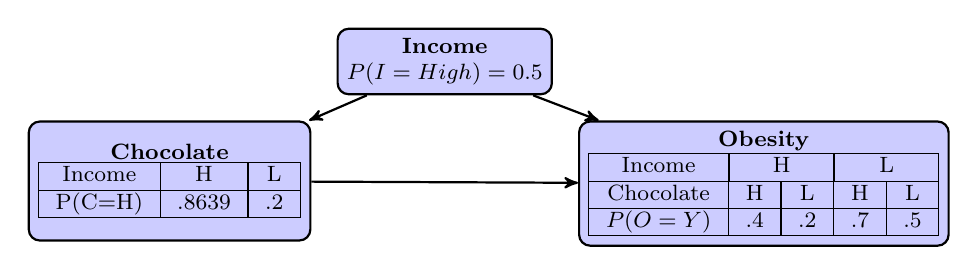
\begin{tikzpicture}[->,shorten >=0pt,shorten <=0pt,node distance=0.45cm,thick,main node/.style={observed}]
\node[main node, align=center,minimum height=4.3em](C){\textbf{Chocolate} \\ \begin{tabular}{| c | c | c |}
  \hline			
  Income & H & L \\
  \hline
  P(C=H) & .8639 & .2\\
  \hline
\end{tabular}};
\node[main node, above right=of C, align=center](I){\textbf{Income} \\ $P(I=High) = 0.5$};
\node[main node, below right=of I, align=center,minimum height=4.3em](O){\textbf{Obesity} \\ \begin{tabular}{| c | c | c | c | c |}
  \hline			
  Income & \multicolumn{2}{| c |}{H} & \multicolumn{2}{| c |}{L} \\
  \hline
  Chocolate & H & L & H & L \\
  \hline
  $P(O=Y)$ & .4 & .2 & .7 & .5 \\
  \hline
\end{tabular}};
\path[]
	(I) edge (C) edge (O)
	(C) edge (O);
\end{tikzpicture}
\end{subfigure}
\begin{subfigure}[t]{0.3\textwidth}
\centering
\caption{Perfect map for $P, \;(C \ci O)$}
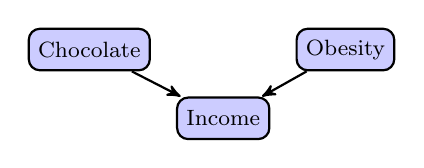
\begin{tikzpicture}[->,shorten >=0pt,shorten <=0pt,node distance=0.45cm,  thick,main node/.style={observed}, shaded/.style={latent}]
\node[main node](C){Chocolate};
\node[main node, below right=of C](I){Income};
\node[main node, above right=of I](O){Obesity};
\path[]
	(C) edge (I)
	(O) edge (I);
\end{tikzpicture}
\end{subfigure}
\end{figure}

\end{document}